\iffalse
\documentclass[12pt]{article}
\usepackage{graphicx}
\usepackage[none]{hyphenat}
\usepackage{graphicx}
\usepackage{listings}
\usepackage[english]{babel}
\usepackage{graphicx}
\usepackage{caption} 
\usepackage{booktabs}
\usepackage{array}
\usepackage{amssymb} % for \because
\usepackage{amsmath}   % for having text in math mode
\usepackage{extarrows} % for Row operations arrows
\usepackage{listings}
\usepackage[utf8]{inputenc}
\lstset{
  frame=single,
  breaklines=true
}
\usepackage{hyperref}
  
%Following 2 lines were added to remove the blank page at the beginning
\usepackage{atbegshi}% http://ctan.org/pkg/atbegshi
\AtBeginDocument{\AtBeginShipoutNext{\AtBeginShipoutDiscard}}


%New macro definitions
\newcommand{\mydet}[1]{\ensuremath{\begin{vmatrix}#1\end{vmatrix}}}
\providecommand{\brak}[1]{\ensuremath{\left(#1\right)}}
\newcommand{\solution}{\noindent \textbf{Solution: }}
\newcommand{\myvec}[1]{\ensuremath{\begin{pmatrix}#1\end{pmatrix}}}
\providecommand{\norm}[1]{\left\lVert#1\right\rVert}
\providecommand{\abs}[1]{\left\vert#1\right\vert}
\let\vec\mathbf

\begin{document}

\begin{center}
\title{\textbf{LINE}}
\date{\vspace{-5ex}} %Not to print date automatically
\maketitle
\end{center}

\section{11$^{th}$ Maths - EXERCISE-10.3}
\begin{enumerate}
\end{enumerate}
\section{SOLUTION}
\fi
Let
Given points are 
\begin{align}
\vec{A}=\myvec{h\\ 3},\vec{B}=\myvec{4\\ 1} 
\implies \vec{B}-\vec{A}=
\myvec{4-h\\ -2}
\end{align}
The given line equation  can be expressed as
\begin{align}
\myvec{7& -9}\vec{x}&=19
\end{align}
yielding 
\begin{align}
\vec{n}=\myvec{7\\ -9},
\vec{m}=\myvec{9\\ 7}
\end{align}
Thus, 
\begin{align}
	\vec{m}^\top\brak{\vec{B}- \vec{A}}&=0\\
\implies\myvec{9& 7}\myvec{4-h\\ -2}&=0\\
\implies h&=\frac{22}{9}
\end{align}
See Fig. 
		\ref{fig:chapters/11/10/3/10/Figure}.
\begin{figure}[h]
\centering
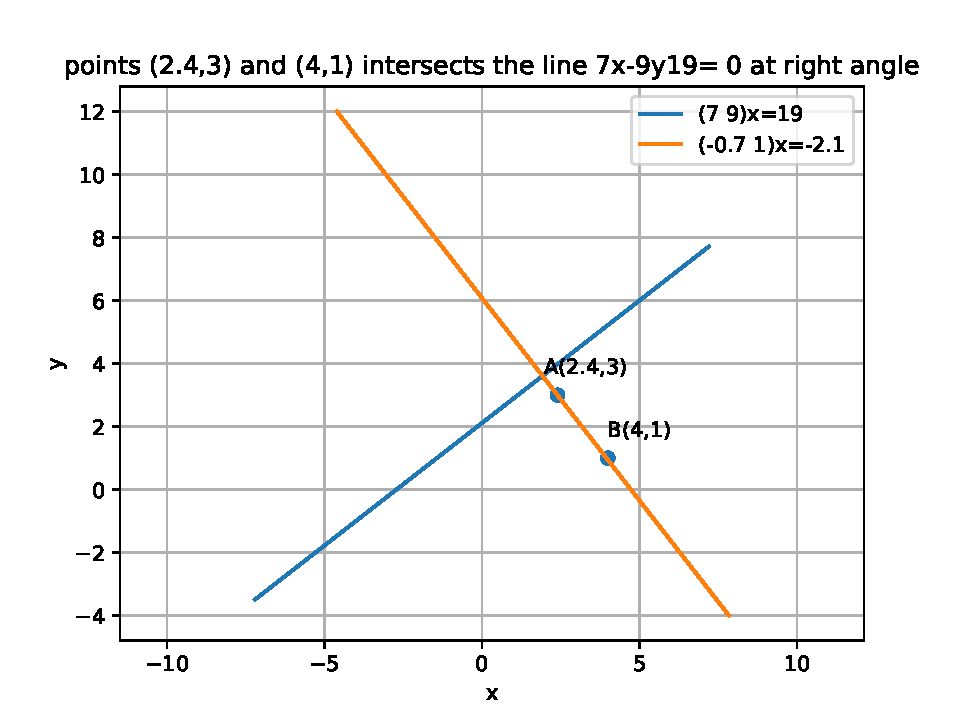
\includegraphics[width=\columnwidth]{chapters/11/10/3/10/figs/fig.pdf}
\caption{}
		\label{fig:chapters/11/10/3/10/Figure}
\end{figure}
